% 第9章第5节：泛函优化的有限维近似（试探空间与Ritz方法、离散目标的构造、误差来源）。

\section{泛函优化的有限维近似}
\label{sec:opt-fn-approximation}

计算机只能处理有限个数。要把泛函优化交给前面各章的算法，必须把候选函数和目标都化成有限维对象。本节分开说明两种化法：限制候选的表示，以及改造目标的计算公式；最后把由此产生的误差按来源区分，因为“算出来的数”同时受到这几种近似的影响。

\subsection{试探空间与Ritz方法}
\label{sec:opt-fn-ritz}

最直接的办法是只在有限个函数张成的集合里找候选。目标的定义保持不变，只是把搜索范围缩小。

\paragraph{有限表示与系数导数}
选择满足必要边界条件的试探函数，写
\[
 u_{\bm a}=u_0+\sum_{j=1}^Na_j\varphi_j,\qquad\bm a\in\mathbb R^N ,
\]
其中$u_0$实现规定的边界值，每个$\varphi_j$的边界值为零，于是每个$u_{\bm a}$都满足本质边界条件。$\varphi_1,\dots,\varphi_N$张成的空间称为\term{试探空间}（trial space）。把泛函限制在这一族上，得到有限维目标$J_N(\bm a)=J(u_{\bm a})$，在其上求最小，这就是\term{Ritz方法}（Ritz method）。映射$\bm a\mapsto u_{\bm a}$是仿射的，由链式法则（定理~\ref{thm:opt-fn-chain-rule}），只要$J$在$u_{\bm a}$处Fréchet可微，
\begin{equation}
 \frac{\partial J_N}{\partial a_j}(\bm a)=DJ(u_{\bm a})[\varphi_j],\qquad j=1,\dots,N .
 \label{eq:opt-fn-ritz-gradient}
\end{equation}
有了~\eqref{eq:opt-fn-ritz-gradient}，就可以调用第~\ref{chap:opt-smooth}章的梯度型或Newton型方法，或在二次目标时直接解线性方程组。

\begin{example}[帽函数上的Ritz方法]
\label{ex:opt-fn-ritz-hat}
在$[0,1]$上最小化$J(u)=\int_0^1\bigl(\frac12u'^2-fu\bigr)\,dx$，$u(0)=u(1)=0$，取$f(x)=\pi^2\sin(\pi x)$。内部方程是$-u''=f$，满足边界条件的解为$u^\star(x)=\sin(\pi x)$；目标凸，与第~\ref{sec:opt-fn-euler-lagrange}节相同的平方差展开说明它是唯一最小点。把区间等分为$N$段，节点$x_j=j\Delta x$，$\Delta x=1/N$，取帽函数
\[
 \varphi_j(x)=\max\Bigl(0,\ 1-\frac{|x-x_j|}{\Delta x}\Bigr),\qquad j=1,\dots,N-1 .
\]
$\varphi_j$在$x_j$处为$1$，在其他节点为$0$，所以系数$a_j$就是$u_{\bm a}$在节点$x_j$处的值；$u_0=0$。代入目标，
\[
 J_N(\bm a)=\frac12\bm a^\top\bm K\bm a-\bm b^\top\bm a,\qquad K_{i,j}=\int_0^1\varphi_i'\varphi_j'\,dx,\quad b_j=\int_0^1f\varphi_j\,dx .
\]
$\varphi_j'$在$x_j$左侧为$1/\Delta x$、右侧为$-1/\Delta x$，于是$\bm K$是对角元$2/\Delta x$、相邻非对角元$-1/\Delta x$的三对角矩阵，对称正定，最小点由$\bm K\bm a=\bm b$唯一确定。

图~\ref{fig:opt-fn-ritz-hat}(a)画出$N=4$与$N=8$的结果：折线的节点值与$\sin(\pi x)$重合。这是本例的特殊性质：由$-u^{\star\prime\prime}=f$分部积分，$b_j=\int_0^1u^{\star\prime}\varphi_j'\,dx=\bigl(2u^\star(x_j)-u^\star(x_{j-1})-u^\star(x_{j+1})\bigr)/\Delta x$，恰好是$\bm K$作用在节点值向量上的第$j$个分量，所以$a_j=u^\star(x_j)$。(b)中，网格每加密一倍，导数误差$\|(u^\star-u_N)'\|_{L^2}$约减半（$N=4,8,16$时约为$0.499$、$0.251$、$0.126$），函数值误差$\|u^\star-u_N\|_{L^2}$约降为四分之一。这是对本例的数值观察；一般条件下离散解收敛的证明属于第~\ref{part:dynamical-systems-control-and-decision}部分。
\end{example}

\begin{figure}[!htb]
  \centering
  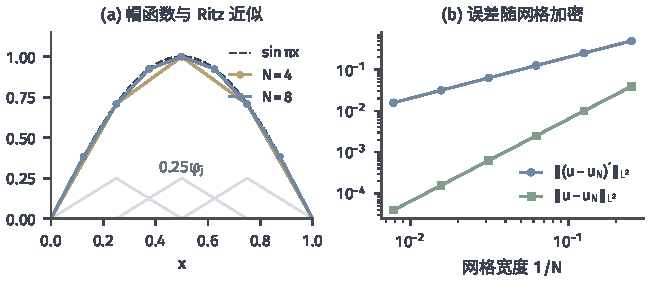
\includegraphics[width=110mm]{figures/03-optimization-evolution-and-signals/01-optimization/matplotlib/c9-ritz-hat/figure.pdf}
  \caption{帽函数试探空间上的Ritz方法，问题为$\min\int_0^1(\frac12u'^2-\pi^2\sin(\pi x)\,u)\,dx$，$u(0)=u(1)=0$，精确解$\sin(\pi x)$（黑色虚线）。(a)~$N=4$时的三个帽函数（灰，缩小为$0.25$倍）及$N=4$（黄）、$N=8$（蓝）的分段线性近似；(b)~$N=4,8,\dots,128$时导数误差（蓝）与函数值误差（绿）随网格宽度的变化，双对数坐标，斜率约为$1$与$2$。误差积分用每段6点Gauss--Legendre求积。}
  \label{fig:opt-fn-ritz-hat}
\end{figure}

\paragraph{改变的是候选集合}
Ritz方法把可行集$C$换成了$C\cap(u_0+\operatorname{span}\{\varphi_j\})$，目标本身没有改变，积分也还没有近似：上例中$\bm K$和$\bm b$都是精确积分。因为可行集变小，$J_N$的最小值不低于原问题的最小值，二者之差就是试探空间的限制误差。返回的函数$u_{\bm a}$需要回到原问题核对约束：本质边界条件由构造保证，其他约束（如非负性）则要另行检查。有限维问题本身是否有解，也须按$J_N$的目标与约束重新判断；上例靠的是$\bm K$正定。

\paragraph{系数梯度与函数梯度}
\eqref{eq:opt-fn-ritz-gradient}给出的是对系数的偏导数，它和按函数内积定义的梯度不同。若要在试探空间中找$L^2$梯度$g=\sum_jc_j\varphi_j$，条件$\langle g,\varphi_i\rangle_{L^2}=DJ(u_{\bm a})[\varphi_i]$写成
\[
 \bm M\bm c=\nabla_{\bm a}J_N(\bm a),\qquad M_{i,j}=\langle\varphi_i,\varphi_j\rangle_{L^2} .
\]
$\bm M$是试探函数的Gram矩阵，在有限元语境中称为\term{质量矩阵}（mass matrix）。帽函数两两不正交，等距网格上$\bm M$是对角元$2\Delta x/3$、相邻非对角元$\Delta x/6$的三对角矩阵。只有基函数关于所用内积标准正交时，$\bm M$才是单位矩阵，系数梯度才等于函数梯度的系数。

\subsection{离散目标的构造}
\label{sec:opt-fn-discrete-objective}

另一种化法不先选试探函数，而是直接把目标中的导数和积分换成有限的差分与求和。这样得到的是一个新的目标，需要单独说明它与原目标的关系。

\paragraph{差分与求和}
从一维导数平方能量$\frac12\int_0^1|u'|^2dx$出发，把区间等分为$N$段，网格宽度$\Delta x=1/N$，节点$x_i=i\Delta x$。在第$i$段上用差商$(u_{i+1}-u_i)/\Delta x$近似导数，再乘以积分单元的长度$\Delta x$，得到
\begin{equation}
 E_N(u)=\frac12\sum_{i=0}^{N-1}\Bigl(\frac{u_{i+1}-u_i}{\Delta x}\Bigr)^2\Delta x=\sum_{i=0}^{N-1}\frac{(u_{i+1}-u_i)^2}{2\Delta x} .
 \label{eq:opt-fn-discrete-energy}
\end{equation}
同一个公式有两种用途。一是固定一个已知函数$u$，取$u_i=u(x_i)$，用$E_N(u)$近似它的能量值；二是把节点值$(u_0,\dots,u_N)$本身当作未知量，在其上优化。后者若再固定$u_0,u_N$，就与上一小节的帽函数Ritz方法重合：分段线性函数在每段上导数恒为差商，$E_N$恰好等于$\frac12\int|u'|^2$。网格不等距时分母要换成各段的宽度；积分权重、边界处理一旦改变，$E_N$就是另一个目标，须重新核算。

\paragraph{点云上的图能量}
没有规则网格时，只有一组点$x_1,\dots,x_n$及其上的取值$u_i$。给定对称非负权重$w_{i,j}=w_{j,i}$，例如由点间距离经核函数算出，定义
\begin{equation}
 E_w(u)=\frac14\sum_{i=1}^n\sum_{j=1}^nw_{i,j}(u_i-u_j)^2=\frac12\sum_{\{i,j\}}w_{i,j}(u_i-u_j)^2 .
 \label{eq:opt-fn-graph-energy}
\end{equation}
左式对有序点对求和，每条无向边被计了两次，所以系数为$\frac14$；右式每条无向边只计一次，系数为$\frac12$，二者相等。写成矩阵，$E_w(u)=\frac12\bm u^\top\bm L\bm u$，其中$\bm L=\bm D-\bm W$，$\bm D$是以$D_{i,i}=\sum_jw_{i,j}$为对角元的对角矩阵。例如三点上$w_{1,2}=1$、$w_{2,3}=2$、$w_{1,3}=0$，取$\bm u=(0,1,3)$，右式给出$\frac12(1\cdot1^2+2\cdot2^2)=4.5$，左式给出$\frac14(2\cdot1+2\cdot8)=4.5$。若要把$E_w$解释为某个连续能量的近似，还需另外给定采样密度、邻近尺度、核权重与样本数的归一化；这些条件不全时，结论只属于图上的离散目标。点云位于曲面上时的几何比较涉及流形，可参考\BookChapterRef{chap:differential-geometry-and-symmetry}{卷四“非线性空间与流形”章}。

\paragraph{改目标与换内积}
回到第~\ref{sec:opt-fn-hilbert-gradient}节的区分。改变网格权重或边权$w_{i,j}$，改变的是目标本身，最小点一般随之改变。固定目标，改用另一个内积计算梯度（例如用$\bm M$或$\bm L+\bm I$代替单位矩阵），改变的是梯度的表示和迭代轨迹，不改变最小点。两种操作在离散公式中都表现为“乘一个矩阵权重”，形式相似，但不能用换内积去补偿一个未经论证的目标离散。

\subsection{误差来源}
\label{sec:opt-fn-error-sources}

一次数值计算交出的结果，同时受三种近似影响：试探空间限制了候选，离散公式改变了目标，有限次迭代没有精确求出离散问题的最小点。比较它们时，每次只改变一个环节，其余固定。

\paragraph{固定函数的能量一致性}
先只看目标离散。下面的结论比较的是同一个已知函数的两个能量值，与优化无关。

\begin{theorem}[差分能量的一致性]
\label{thm:opt-fn-energy-consistency}
设$u\in C^1[0,1]$，$u_i=u(x_i)$，则$N\to\infty$时$E_N(u)\to\frac12\int_0^1u'(x)^2\,dx$。
\end{theorem}

\begin{proof}
由中值定理，每段上存在$\xi_i\in(x_i,x_{i+1})$使$(u_{i+1}-u_i)/\Delta x=u'(\xi_i)$，所以$E_N(u)=\frac12\sum_iu'(\xi_i)^2\Delta x$。这是连续函数$u'^2$在$[0,1]$上的一个Riemann和。$u'^2$在闭区间上一致连续：对任意$\varepsilon>0$，当$\Delta x$足够小时，同一段内任两点处$u'^2$之差小于$\varepsilon$，于是Riemann和与积分之差不超过$\varepsilon$。
\end{proof}

取$u=\sin(\pi x)$可以算出精确值。由$\sin\alpha-\sin\beta=2\cos\frac{\alpha+\beta}2\sin\frac{\alpha-\beta}2$及$\sum_{i=0}^{N-1}\cos^2\bigl(\pi(i+\frac12)/N\bigr)=N/2$（$N\ge2$），
\[
 E_N(\sin\pi x)=N^2\sin^2\frac\pi{2N}=\frac{\pi^2}4-\frac{\pi^4}{48N^2}+O(N^{-4}) .
\]
图~\ref{fig:opt-fn-energy-consistency}显示，$N=2$时$E_N=2$，$N=8$时约为$2.436$，误差随$N^{-2}$下降。定理只说明固定函数的能量值收敛，它还没有比较两个优化问题的最小点：离散最小点是否收敛到连续最小点，需要另外的稳定性与逼近条件。

\begin{figure}[!htb]
  \centering
  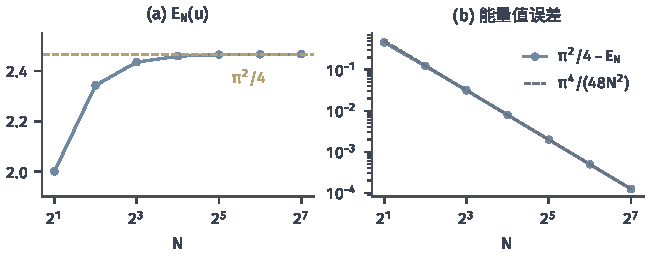
\includegraphics[width=110mm]{figures/03-optimization-evolution-and-signals/01-optimization/matplotlib/c9-energy-consistency/figure.pdf}
  \caption{固定函数$u=\sin(\pi x)$的差分能量~\eqref{eq:opt-fn-discrete-energy}。(a)~$E_N(u)=N^2\sin^2(\pi/(2N))$随$N=2,4,\dots,128$趋于$\pi^2/4\approx2.467$（黄色虚线）；(b)~误差$\pi^2/4-E_N$（蓝）与渐近式$\pi^4/(48N^2)$（灰色虚线）几乎重合，双对数坐标。}
  \label{fig:opt-fn-energy-consistency}
\end{figure}

\paragraph{边权扰动的目标值界}
对点云上的固定记录$\bm u$，同一计数口径下只改变边权，从$w$换成$\widetilde w$。逐项相减，
\[
 \bigl|E_w(u)-E_{\widetilde w}(u)\bigr|\le\frac14\sum_{i,j}|w_{i,j}-\widetilde w_{i,j}|(u_i-u_j)^2 .
\]
上面的三点例子中，把$w_{1,2}$从$1$改为$1.1$（$w_{2,1}$随之改变），右边为$\frac14\cdot2\cdot0.1\cdot1=0.05$，而$E_{\widetilde w}(u)=4.55$，差恰为$0.05$。这个界是同一记录上的目标值扰动界。若两个目标各自重新优化，最小点之间相差多少还依赖强制性、唯一性或其他稳定性条件，不能从这个不等式直接读出。

\paragraph{报告数值结果时}
迭代停止时，宜把三件事分开核验：离散目标是否已充分下降（例如梯度范数或对偶间隙）；返回的函数是否保留了原问题的约束；所用离散目标是否在相关函数上一致地近似连续目标。能量值的一致性、连续最小点的存在、离散最小点的收敛与求解器的收敛是四个不同的命题。本章分别给出了第一个的简单情形与第二个的直接法；具体方程的网格解收敛，由第~\ref{part:dynamical-systems-control-and-decision}部分在相应的一致性、稳定性与逼近条件下建立。
